\chapter{Planteamiento del Problema}
\section{Descripción de la Realidad Problemática}

Hoy en día, la producción de papa es una de las actividades más importantes en nuestro país tanto a nivel económico como alimenticio y el Perú es el mayor productor de papa en América Latina contando con más de 4mil variedades.\parencite{cr_elcomercioproduccionpapa}.  


De acuerdo al reporte del Ministerio de Desarrollo Agrario y Riego (Midagri) del 2023, el consumo de papa por persona es de, aproximadamente, 92 kilos por año, cifra que ha venido incrementándose desde hace dos décadas debido a la importancia que tiene este tubérculo en la dieta de los peruanos. La papa es considerada uno de los alimentos más importantes y nutritivos en el Perú, rico en carbohidratos, proteínas, vitaminas y minerales.  Mientras que otros productos relevantes como el arroz no se cultivan en más de 7 regiones, lo que evidencia la amplia distribución geográfica del cultivo de papa en el territorio peruano \parencite{cr_agroinforma1}. Asimismo, el tubérculo se siembra en 19 distintas regiones del país, resaltando en departamentos como Puno y Huánuco, que lideran la producción nacional con 20.6\% y 12.6\% respectivamente \parencite{minagri_estadisticas_2022}. También, según el Censo Nacional Agropecuario 2022, el cultivo de papa es el sustento de al menos 710,000 familias en el Perú, representando aproximadamente el 25\% de los hogares dedicados a la agricultura y aportando el 6.5\% al PBI agropecuario del país \parencite{inei_cenagro_2022}.
 
 Sin embargo, el los últimos años, la producción se ha visto afectada por una de las patologías más mortales que es Phytophthora infestans, conocido por los agricultores como Rancha o tizón tardío, la cual es capaz de acabar con el 100\% de cultivos enteros en solo unos días sino se antepone una medida de prevención. Según el técnico del Servicio para el Desarrollo Integral Rural,   la rancha es peligrosa y puede arruinar  toda la siembra. Es relevante para el agricultor diagnosticarla y encontrar la mejor manera de controlarla. Las condiciones climáticas propicias para la aparición de la rancha o tizón tardío se dan cuando las temperaturas fluctúan entre los 15°C y 18°C, o bien, cuando la temperatura se mantiene por debajo de los 25°C durante un periodo de 7 días consecutivos. Asimismo, esta enfermedad se ve favorecida por la presencia de lluvias constantes o cuando los niveles de humedad relativa oscilan entre el 90\% y el 100\% \parencite{cr_rancha1}. Los principales síntomas de la enfermedad en el tubérculo son: hojas, lesiones en los bordes mostrando manchas necróticas con halo amarillento y micelio blanquecino en el relieve de la hojas; tallos, lesiones que recorren el tallo de color marrón osucro; tubérculos, lesiones irregulares en de color marrón rojizo que no solo están presentes en los alrededores de la papa sino del al interior también \parencite{cr_rancha2}. . El caso más popular sobre rancha en Perú ocurrió en 2010 afectando a la región de Junín, donde al menos 26 mil de toneladas de papa fueron afectadas por la rancha en dos mil 660 hectáreas , lo cual representó una pérdida de 10 millones de nuevos soles. Esto se pudo evitar con fungicidas; sin embargo, estos son costosos entonces no todos los agricultores tiene accesso a este \parencite{cr_rancha6}. 
 
 En abril de 2024, la rancha afectó a sembríos de papa nativa en la sierra de Lima, según resportes el tizón tardío arrasó con tres custodios de papa autóctonos tres en Huarachorí, dos en Yauyos y uno en Cajatambo \parencite{cr_rancha3}. Asimismo, en marzo de 2024, la rancha afectó fuertemente en el departamento de Junín, haciendo que 2000 agricultores pierdan, aproximadamente, 550 héctareas de papa por el tizón tardío, valorizando esta pérdida en S/300 mil. Siendo este el principal cultivo agricola en su sierra \parencite{cr_rancha4}. Finalmente, en abril de 2024, la rancha atacó el departamento de Apúrimac, la cual perdió una hectárea de papa y una y media hectáreas de cultivos afectados \parencite{cr_rancha5}.
 
 Ante esto, el gobierno se ha visto obligado a concientizar sobre la rancha, en marzo de 2024, el Servicio para el Desarrollo Integral Rural (Sedir) y Servicio Nacional de Sanidad Agraria (Senasa) en Ancash, ya que varios agricultores locales temen perder sus sembríos debido a la rancha, principalmente porque se desarolla en temperaturas entre 12°C y 16°C y con fuerte presencia de humedad. Según la charla, una forma de prevenir la rancha es rotando el cultivo, es decir cambiando a otros productos como maíz y alverja \parencite{cr_agroinforma2}.
 
 Por eso mismo, con el gran avance de la Inteligencia Artificial (IA) se ha perfeccionado y popularizado su uso en el sector agrícola de distintas formas, ya que es una herramienta útil y apta para procesar enormes cantidades de información rápidamente. . La IA es una alternativa tecnología que puede brindar soluciones prácticas porque es eficiente creando algoritmos capaces de detectar patologías a tiempo, así como mejorar tanto la precisión del diagnóstico como la eficiencia del flujo de trabajo en el campo, además que reduce costes porque agiliza. La IA también se puede emplear para identificar a plantas que están en peligro de pescar una enfermedad específica, lo que facilita la intervención y prevención temprana. Por ejemplo, un estudio reciente mostró que un sistema de IA logró detectar la zona enferma de una hoja con una precision deñ 96.44\% \parencite{cr_iaplanta}.
 
 Añadiendo, la adopción de tecnología de IA en el ámbito de la agricultura del Perú puede ofrecer soluciones para una serie de problemas que enfrenta el sistema de siembra y cosecha, como el bajo acceso a asistencia técnica  en este sector en el país, la escasez de personal, la falta de competencias y la insuficiencia de equipos tecnológicos para una mejor desempeño para el proceso agrícola. En muchas ocasiones, particularmente en las zonas rurales y de recursos limitados, la falta de tecnología agrícola adecuada puede restringir la productividad y la calidad de los cultivos en la agricultura peruana. Sin embargo, al emplear herramientas de inteligencia artificial, como sistemas de monitoreo automatizado de cultivos y análisis de datos agrícolas, se puede incrementar la eficiencia en la producción, reducir los costos y garantizar una mayor calidad de los productos agrícolas, beneficiando así a más agricultores y contribuyendo al desarrollo sostenible del sector.En muchos casos, especialmente en las áreas rurales y de bajos ingresos del Perú, la falta de equipamiento agrícola básico y adecuado limita el rendimiento y la productividad de los cultivos. Al utilizar herramientas de inteligencia artificial, como sistemas de monitoreo de cultivos, análisis de patologías en cultivos y predicción del clima, se puede mejorar la toma de decisiones en cuanto a la siembra, el riego y la aplicación de insumos, optimizando los recursos y aumentando los rendimientos, lo que permite una mayor producción agrícola para alimentar a más personas. Un porcentaje significativo de los trabajos se enfocan en la detección y diagnóstico de enfermedades (29.4\%) y en la recomendación de fertilizantes (29.4\%), sin embargo, este último aspecto no abarca específicamente el cultivo de maíz. Los sistemas expertos están diseñados principalmente para que el agricultor pueda tomar decisiones más acertadas durante el ciclo de cultivo, lo cual representa el 80.6\% de los casos. Estos sistemas se consideran usuarios potenciales, ya que muchos agricultores no tienen los recursos para contratar a un experto en el área. Los sistemas expertos ofrecen una alternativa accesible y de bajo costo \parencite{cr_iaplanta2}. 
 
En este contexto, el desarrollo de un sistema de visión computacional que utilice técnicas de inteligencia artificial y aprendizaje automático para detectar y clasificar la rancha o tizón tardío de forma temprana en las hojas de papa peruana se presenta como una solución prometedora. Mediante el análisis automatizado de imágenes de las hojas, este sistema podría identificar con alta precisión los síntomas iniciales de la enfermedad, permitiendo a los agricultores tomar medidas preventivas oportunas y evitar mayores pérdidas en sus cultivos. La visión computacional, al ser una tecnología no invasiva, económica y escalable, se perfila como una herramienta valiosa para abordar este desafío fitosanitario que amenaza la producción y la seguridad alimentaria en el Perú. Al integrar algoritmos avanzados de reconocimiento de patrones y clasificación de imágenes, este sistema tendría el potencial de mejorar significativamente el diagnóstico precoz de la rancha, contribuyendo así a la sostenibilidad del sector papero, pilar fundamental de la agricultura y la economía familiar en diversas regiones del país.

En este sentido, la presente investigación busca desarrollar e implementar un sistema robusto y escalable de visión computacional, aprovechando los avances tecnológicos más recientes, con el fin de proporcionar una solución innovadora, accesible y de alto impacto para los agricultores peruanos, facilitando la lucha contra esta devastadora enfermedad y promoviendo la resiliencia y productividad de los cultivos de papa a nivel nacional.
 %\medskip

%\begin{figure}[h]
%	\begin{center}
%		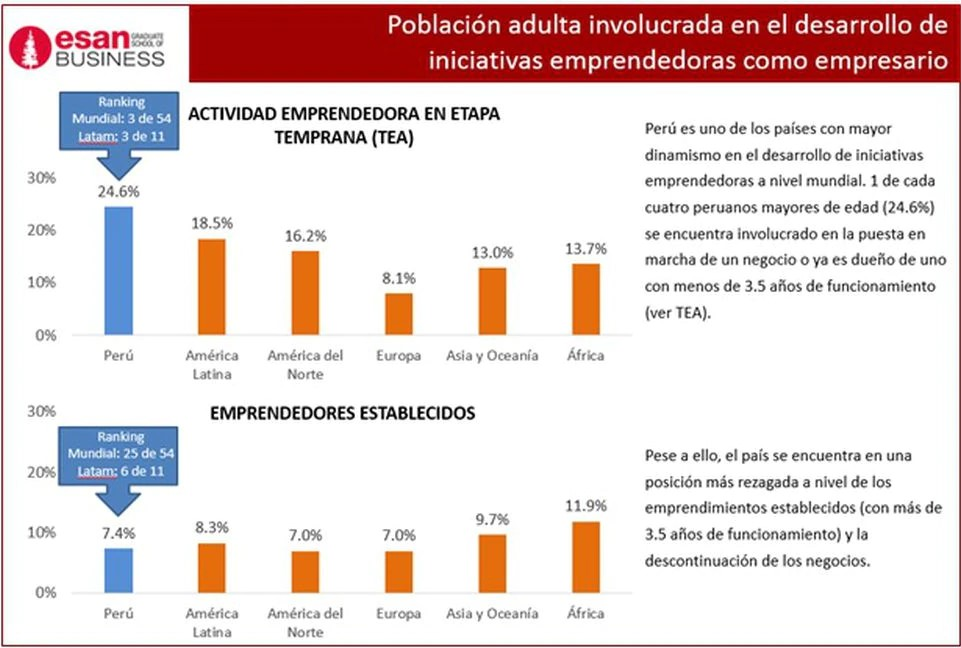
\includegraphics[width=0.65\textwidth]{1/figures/cuadro_esan.jpg}
%		\caption[Resultados y ratios obtenidos en la encuesta por GEM y %ESAN]{Resultados y ratios obtenidos en la encuesta por GEM y ESAN.\\
%		Fuente: \cite{cr_gestion2018emprend}. \textit{Perú es el tercer país con %mayor cantidad de emprendimientos en fase temprana a nivel mundial}.}
%		\label{1:fig}
%	\end{center}
%\end{figure}


%\begin{figure}[h]
%	\begin{center}
%		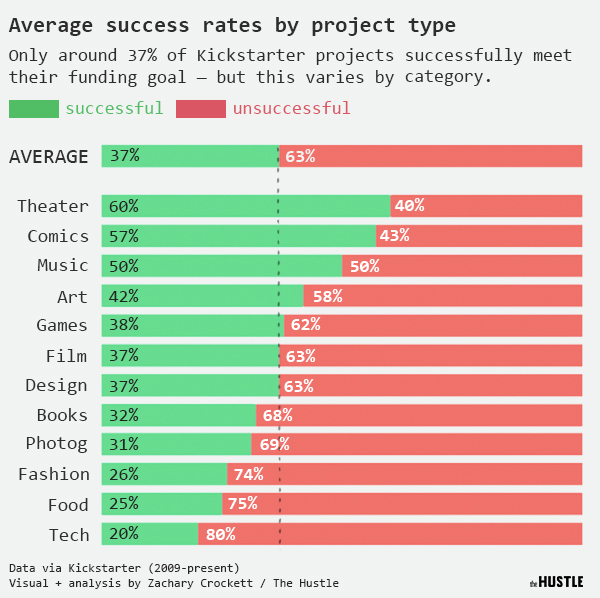
\includegraphics[width=0.55\textwidth]{1/figures/kickstarter_success_rate_2009_2019.jpg}
%		\caption[Ratio de éxito de proyectos en Kickstarter desde 2009 hasta 2019 %(Febrero)]{Ratio de éxito de proyectos en Kickstarter desde 2009 hasta 2019 (Febrero).\\
%		Fuente: \cite{cr_hustle2019successrate}. \textit{What are your chances of successfully %raising money on Kickstarter?}}
%		\label{1:fig2}
%	\end{center}
%\end{figure}


\section{Formulación del Problema}
Para la formulación de los problemas de la presente investigación, se elaboró un «árbol de problemas» (véase Anexo \ref{anexo1}).

\subsection{Problema General}
PG: \newcommand{\ProblemaGeneral}{
	¿Es posible desarrollar un sistema de visión computacional que permita la clasificación temprana de la rancha (Phytophthora infestans) en hojas de papa peruana con alta precisión?
}
\ProblemaGeneral

\subsection{Problemas Específicos}
\newcommand{\Pbone}{
	¿Cómo podemos desarrollar un sistema de clasificación automática de "Rancha" Phytophthora infestans en las hojas de papa peruana que sea preciso, eficiente y robusto a la variabilidad de las lesiones y las condiciones ambientales?
	
}

\newcommand{\Pbtwo}{
¿Cómo implementar técnicas de aprendizaje automático para clasificar las manchas detectadas como síntomas de Rancha o no, con una alta precisión y anticipación?
}

\newcommand{\Pbthree}{
 ¿Cómo desarrollar un método de segmentación preciso que permita separar las manchas de Rancha de otros elementos presentes en las hojas de papa, como venas y áreas sanas?
}

\newcommand{\Pbfour}{
¿Cómo reducir el tiempo de procesamiento requerido para analizar grandes volúmenes de imágenes de hojas de papa y proporcionar resultados de detección y clasificación en tiempo real o con una rápida respuesta?
}


\begin{itemize}
	\item PE1: {\Pbone}
	\item PE2: {\Pbtwo}
	\item PE3: {\Pbthree}
	\item PE4: {\Pbfour}
\end{itemize}

\section{Objetivos de la Investigación}

\subsection{Objetivo General}
OG: \newcommand{\ObjetivoGeneral}{
	Desarrollar un sistema de visión computacional basado en técnicas de aprendizaje profundo para la clasificación temprana de la rancha (Phytophthora infestans) en hojas de papa peruana.
}
\ObjetivoGeneral

\subsection{Objetivos Específicos}
\newcommand{\Objone}{
Desarrollar un sistema de clasificación automática de "Rancha" Phytophthora infestans que alcance una precisión superior al 95\% en la identificación y clasificación de lesiones en las hojas de papa.
}

\newcommand{\Objtwo}{
Entrenar un modelo de aprendizaje automático capaz de clasificar las manchas detectadas como síntomas de Rancha o no, utilizando un conjunto de datos etiquetado.
}

\newcommand{\Objthree}{
Investigar y desarrollar un método de segmentación avanzado que permita una separación precisa de las manchas de Rancha en las hojas de papa, minimizando la interferencia de otros elementos.
}

\newcommand{\Objfour}{
Optimizar los algoritmos desarrollados para reducir el tiempo de procesamiento y mejorar la eficiencia computacional, permitiendo un análisis rápido de grandes conjuntos de datos de imágenes.
}

\begin{itemize}
	\item OE1: {\Objone}
	\item OE2: {\Objtwo}
	\item OE3: {\Objthree}
	\item OE4: {\Objfour}
\end{itemize}

\section{Hipótesis}

\subsection{Hipótesis General}
HG: \newcommand{\HipotesisGeneral}{
Se hipotetiza que mediante el desarrollo de un sistema de clasificación automática de las lesiones de "Rancha" Phytophthora infestans en las hojas de papa peruana, se puede lograr un método de clasificar la Rancha en las hojsa de papa peruana.
}
\HipotesisGeneral
\subsection{Hipótesis Específicas}
\newcommand{\Hone}{
La implementación de técnicas de aprendizaje automático y segmentación de imágenes permitirá desarrollar un sistema de clasificación automática de "Rancha" Phytophthora infestans con alta precisión.
}
\newcommand{\Htwo}{
La aplicación de algoritmos de aprendizaje automático para clasificar las manchas detectadas permitirá una identificación temprana y precisa de la Rancha, mejorando significativamente la capacidad de respuesta ante esta enfermedad en los cultivos de papa.
}
\newcommand{\Hthree}{
 Un método de segmentación avanzado permitirá una separación precisa de las manchas de Rancha, mejorando la precisión del sistema de detección y clasificación.
}
\newcommand{\Hfour}{
 La optimización de los algoritmos para la eficiencia computacional permitirá un procesamiento rápido de las imágenes, facilitando la implementación en sistemas de monitoreo en tiempo real.
}

\begin{itemize}
	\item HE1: \Hone
	\item HE2: \Htwo
	\item HE3: \Hthree
	\item HE4: \Hfour
\end{itemize}

Los problemas, objetivos e hipótesis descritas anteriormente se encuentran alineados en la Matriz de Consistencia del Anexo \ref{anexo3}. Además, los objetivos específicos se formularon a partir de una lluvia de ideas luego de examinar los objetivos planteados en los antecedentes, cuyo detalle e item de referencia se encuentra en el Anexo \ref{anexo5}.

\section{Justificación de la Investigación}

\subsection{Teórica}
El propósito de esta investigación es contribuir al avance en la clasificación temprana de la 'Rancha' Phytophthora infestans en las hojas de papa peruana mediante la aplicación de técnicas de Visión Computacional. Este problema reviste importancia debido a su impacto en la agricultura peruana, donde la detección temprana de la enfermedad es crucial para su manejo efectivo.

Cabe recalcar que cada vez este tipo de herramientas tecnológicas son más útiles para la clasificacion de patologias visuales en las hojas de plantas. Asimosmo, es importante resaltar que no hay este tipo de investigaciones en Perú, siendo uno de los países con más historia con la papa y que cuenta con miles de variedades.

Al implementar este enfoque multimodal, se espera proporcionar una herramienta útil para los agricultores y expertos en la detección temprana de la 'Rancha' Phytophthora infestans, lo que eventualmente podría contribuir a una mejor gestión de esta enfermedad y a la protección de los cultivos de papa en el Perú. 
\subsection{Práctica}
Muchos de los trabajos previos, superaron su efectividad y precision esperada; sin embargo, en gran mayoría de la literatura mencionada (5 de 5) utilizaron técnicas comunes y antiguas, ninguno optó por utilizar técnicas innovadoras como Visual Transformer que en este caso sí se dará.


Al concluior esta investigación, las personas podrán hacer uso del sistema de clasificación temprana de la 'Rancha' Phytophthora infestans en las hojas de papa peruana con el fin de tomar las medidas apropiadas para su control y erradicación. De encontrarse, con una plantación infectada deberán utilizar pesticidas especializados para esos casos de manera profesional. Los beneficiados serán aquellas personas que viven de la cultivación de este tubperculo, tales como agriculturos, campesinos, negociantes y el consumidor final. Esta investigación va a servir para evitar un tardía reacción a la Rancha en los cultivos de papa para que así no haya pérdida de cosecha. El trabajo presente demostrará que un sistema de vision computacional puede clasificar, mediante imágenes RGB de hojas de planta de papa, si el tubérculo presenta la enfermedad de tizón tardío, lo cual puede cambiar el proceso de cuidado de cultivo y no solo del agricultor sino de toda la caneda que se beneficia de este producto.

\subsection{Metodológica}
La implementación del modelo propuesto ayudará a agricultores a clasificar tempranamente el tizón tardío en la papa haciendo su trabajo más rápido y eficiente, ya que una detección temprana promete ser una rápida toma de decisiones que ayudará solucionar y controlar este problema.

Para ello, se utilizaron técnicas Vision Computacional entrenados con un conjunto de datos compuesto por distintas bases de datos reales luego de un proceso de recolección de datos.

\section{Delimitación del Estudio}

\subsection{Espacial}
Para la presente investigación, se consideraron proyectos de tecnología de distintas ciudades y países, mayoritariamente del territorio de lationamericano. Sin embargo, la información textual (descripción y comentarios) para la fase de entrenamiento solo se tómo en cuenta palabras en inglés.

\subsection{Temporal}
El periodo de tiempo abarcará desde el año 2019, fecha en el cual se tiene registrado los primeros conjuntos de datos de proyectos en Kickstarter hasta el mes de agosto del año 2024, últimos registros descargados hasta el inicio del presente trabajo. Asimismo, obtener nuevos algoritmos y resultados que validen que las mismas técnicas pueden ser aplicadas en diferentes contextos.

\subsection{Conceptual}
Esta investigación se orientará en la implementación de un modelo que logre clasificar si un una o varias hojas de papa están infectadas con rancha. Para ello, se valió del uso de herramientas de Vision computacional  para desarrollar los modelos de acuerdo a sus modalidades respectivas.